\documentclass{ctexart}
\begin{document}
\title{计算物理作业 10}
\author{刘畅, PB09203226}
\maketitle

{\bf [作业10]}: 计算 2 维正方格子中 GSAW 的指数值, 并定性地加以讨论.

\section{算法和程序}
我们的程序是要模拟 GSA 随机游走的过程. 这个随机游走发生在一个二维网格上. 为了
在计算机中表示这个二维网格, 一个最简单的想法就是用一个二维 \verb|bool| 数组.
\verb|true| 表示这个格点已经走过, \verb|false| 表示这个格点还没有被走过.
这个二维矩阵是 \verb|dim|$\times$\verb|dim| 大小的, 这个 \verb|dim| 是可变的,
所以要在堆上分配: (\verb|gsa_walk()|)
\begin{verbatim}
  bool (*lattice)[dim] = malloc(dim * dim * sizeof(bool));
\end{verbatim}

算法的核心步骤在于, 在已经给定了行走的历史 (\verb|last_x| 和 \verb|last_y|)
的情况下, 如何选择下一步行走. 如果直接按照
书上的算法用一大堆 \verb|if-then-else| 语句, 程序代码比较乱. 我们要避免这种
做法, 为此我们将四个方向的移动方式放在 \verb|delta_{x,y}[]| 数组中:
(\verb|take_next_step()|)
\begin{verbatim}
  int delta_x[4] = {0, 0, 1, -1}; /* 0 -- up, 1 -- down */
  int delta_y[4] = {1, -1, 0, 0}; /* 2 -- right, 3 -- left */
\end{verbatim}
我们的算法是首先判断上下左右四个方向的格点是否被占用, 将这一信息储存在 \verb|occupied[]|
数组中:
\begin{verbatim}
    bool occupied[4] = {false, false, false, false};
    /* check for possible next directions */
    for (i = 0; i < 4; i++) {
        new_x = last_x + delta_x[i];
        new_y = last_y + delta_y[i];
        if ( (new_x < 0) || (new_x >= dim)
             || (new_y < 0) || (new_y >= dim)
             || (lattice[new_x][new_y] == true) ) {
            occupied[i] = true;
        } else {
            occupied[i] = false;
        }
    }
\end{verbatim}
初始的时候所有的 \verb|occupied[i]| 都是 \verb|false|, 如果被占用, 对应的
\verb|occupied[i]| 就变成 \verb|true|.

接下来我们计算有多少可能的方向, 如果没有方向可走, 这个算法就结束, 返回 \verb|false|:
\begin{verbatim}
    /* count possible next directions */
    nrway = 0;
    for (i = 0; i < 4; i++) {
        if (!occupied[i])
            nrway++;
    }
    /* die if no step could be taken */
    if (nrway == 0)
        return false;
\end{verbatim}

如果有方向可走, 接下来要做的就是等概率地在这些可能的方向中选取一个, 作为下一步
行走的方向. 为此需要在集合 $S = \{i\mid{\rm occupied}[i] \equiv{\rm false}\}$
上的均匀分布中抽样的例程:
\begin{verbatim}
int sample_uniform(bool occupied[4])
{
    int idx;

    do {
        idx = (int) (rand_norm() * 4.0);
    } while (occupied[idx]);

    return idx;
}
\end{verbatim}
这个抽样算法是典型的舍选法, 如果抽到 \verb|occupied[i] == true| 的 \verb|i|,
就把这次抽样舍去, 重新抽样.

有了这个抽样例程, 就可以选取下一步行走的方向了: (\verb|take_next_step()|)
\begin{verbatim}
    /* else take the next step and live strong */
    i = sample_uniform(occupied);
    new_x = last_x + delta_x[i];
    new_y = last_y + delta_y[i];
    lattice[new_x][new_y] = true;
    *plast_x = new_x;
    *plast_y = new_y;
    return true;
\end{verbatim}
这样 \verb|take_next_step()| 例程就编写好了.

接下来就要编写真正做 GSA 随机行走的例程了. 例程在 \verb|gsa_walk()|. 首先要
把 \verb|lattice[][]| 初始化为 \verb|false|.
\begin{verbatim}
    /* initialize lattice to false */
    for (i = 0; i < dim; i++) {
        for (j = 0; j < dim; j++) {
            lattice[i][j] = false;
        }
    }
\end{verbatim}
这个没什么好解释的. 然后要设置行走的初始条件:
\begin{verbatim}
    alive = true;
    last_x = last_y = dim / 2;
    lattice[last_x][last_y] = true;
    asteps = 0;
    sum_r2 = 0;
\end{verbatim}
初始时 \verb|alive| 为真, 表明可以走下一步. \verb|last_x| 和 \verb|last_y|
设在格点中心. \verb|asteps| 表示走了多少步, \verb|sum_r2| 是为了计算
$\langle r^2\rangle$ 所用的变量.

最后最主要的是一个循环, 如果还有方向可走并且没有走到要求的步数, 那么调用前面的
\verb|take_next_step()|, 进行下一步行走, 并且计算和记录相关数据.
\begin{verbatim}
    while (alive && asteps < nsteps) {
        fprintf(fout, "%d %d\n", last_x, last_y);
        sum_r2 += pow(last_x - dim/2, 2)
            + pow(last_y - dim/2, 2);
        alive = take_next_step((bool *) lattice, dim,
                       &last_x, &last_y);
        asteps++;
    }
\end{verbatim}
这样 GSA 随机行走的例程就编写好了.

\section{结果}
首先我们作出一次随机游走的图形, 作图的代码很简单, 直接调用 \verb|gsa_walk()|
就可以了. 代码在 \verb|main.c|. 结果:
\begin{center}
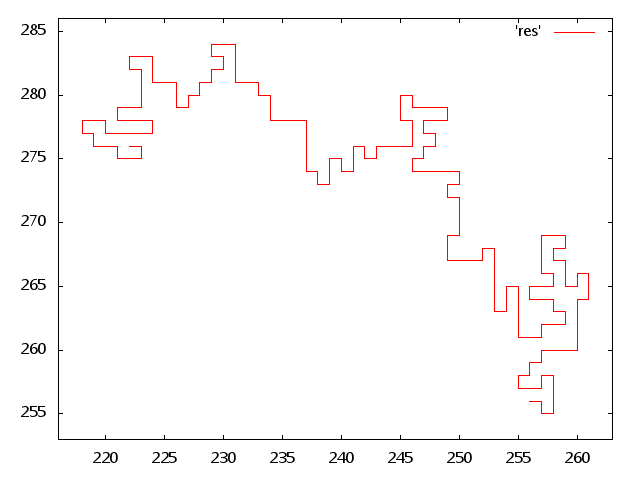
\includegraphics[width=4in]{res.png}
\end{center}

由于这个问题中, 走了几步后, 很大的概率会绕道一个死胡同中, 算法不能进行下去.
因此通常实际步数 \verb|asteps| 是随机的. 我们可以作出它的分布:
\begin{center}
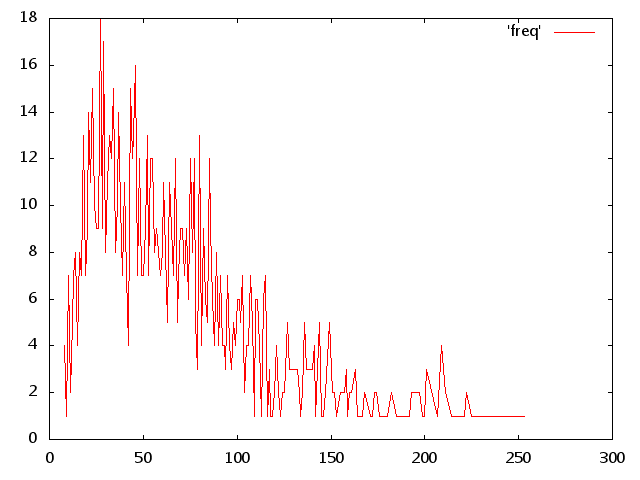
\includegraphics[width=4in]{freq.png}
\end{center}
这个分布比较像 $\Gamma$ 分布的概率分布曲线.
\begin{center}
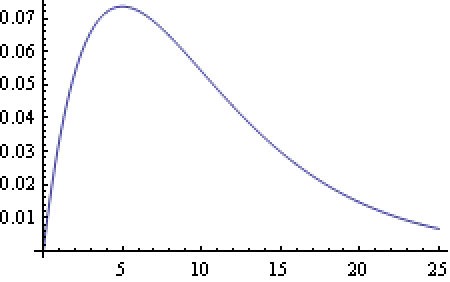
\includegraphics[width=3in]{GammaDistribution.png}
\end{center}

最后我们最关心的问题是 GSAW 的指数值. 为此我们计算 $\langle r^2\rangle$,
并把 $\ln\langle r^2\rangle$ 对 $\ln N$ 做在一张图上.
\begin{center}
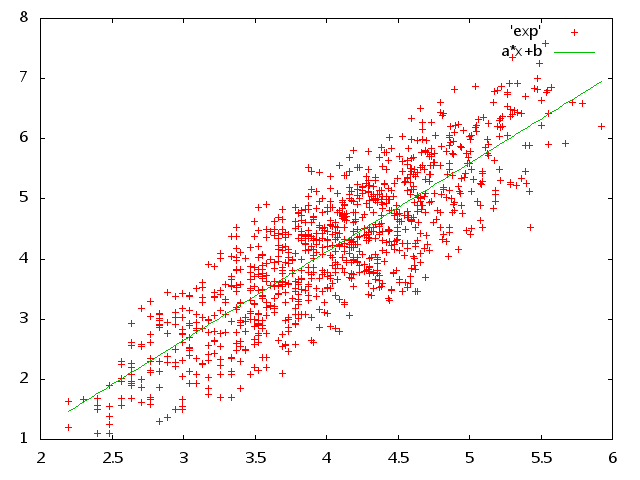
\includegraphics[width=4in]{exp.png}
\end{center}
拟合这个曲线, 得到的斜率的一半就是我们要求的指数. 图上的绿线就是拟合曲线.
得到的指数结果:
\[
\nu=\input res_exp\relax
\]
这个值每次运行程序都不太同, 但都在在 $0.72$ 左右. 比 SAW 的指数 $0.75$ 要小. 

\end{document}